\section{Observation and Calculations}

\subsection{Calibration of Magnetic Field with Coil Current}
By placing the probe inside the electromagnet of 500 turns, we obtain a linear relationship between the current supplied and the magnetic field $\vv{H}$ between the electromagnets (Table \ref{tab:cal}, Fig. \ref{calf}).

\begin{table}[H]
    \centering
    \begin{tabular}{|c|c|c|}
    \hline
    Source & Energy (keV) & Peak Channel \\ \hline
    Ba-133 & 356 & 169.9308 \\ \hline
    Cs-137 & 662 & 302.922 \\ \hline
    Co-60 & 1172 & 525.6078 \\ \hline
    Co-60 & 1335 & 598.9153 \\ \hline
    \end{tabular}
    \caption{Known energy sources calibrated across a range of 1024 channels}
    \label{tab:cal}
    \end{table}
\begin{figure}[H]
    \centering
    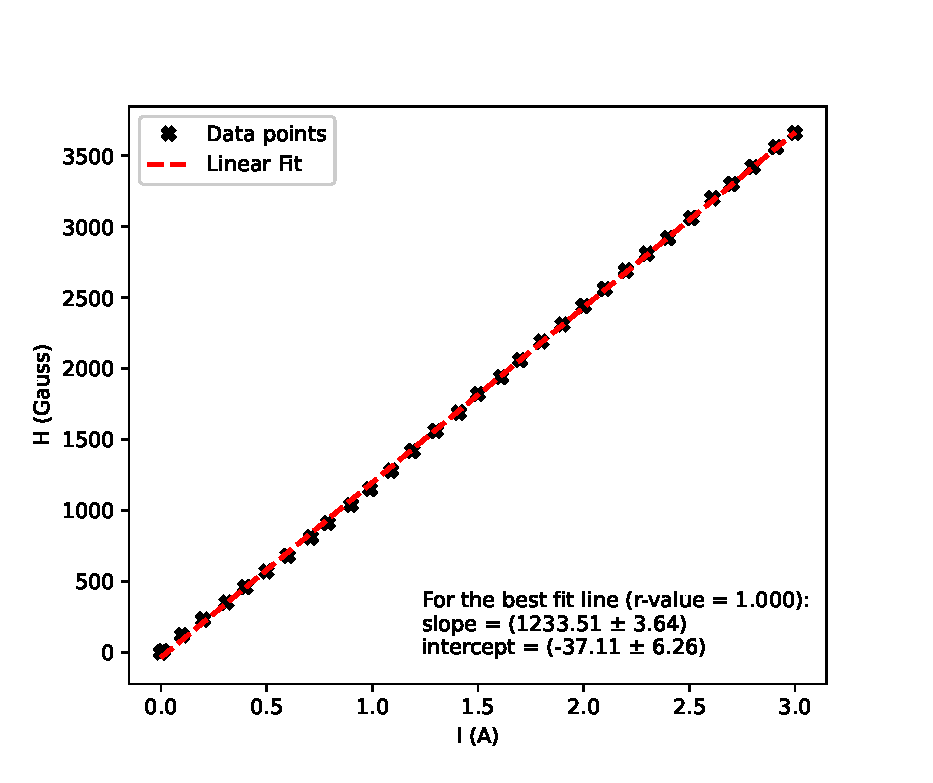
\includegraphics[width=1\columnwidth]{images/cal.eps}
    \caption{Calibration plot for Magnetic field vs. Coil Current}
    \label{calf}
\end{figure}

\subsection{Estimation of Hall Coefficient}

At constant room temperature, we measured the Hall voltage at different values of coil currents for three different semiconductors. 
$H$ was calculated for each $I$ from using $H = (1233.51\cdot I - 37.11)$ Gauss (Fig. \ref{calf}).
\vspace{-1em}
\subsubsection{Ge p-type}
The Hall voltage against different values of coil currents is shown in Table \ref{tab:geP}. The Hall voltage as a function of the magnetic field obtained through the calibration curve plot is shown in Fig. \ref{fig:geP}.

\begin{itemize}
    \item Probe current = 4.31 mA
    \item Resistivity $\sigma = (7 \pm 1)\,\Omega$ cm 
    \item Sample thickness $t= 0.5$ mm
\end{itemize}
\begin{table}[H]
    \centering
    \begin{tabular}{|c|c|c|c|}
    \hline
    Current & Hall Voltage & Current & Hall Voltage \\ 
    (A) & (mV) & (A) & (mV) \\ \hline
    0.01 & 6.3 & 2.00 & 35.0 \\ \hline
    0.10 & 7.9 & 2.10 & 36.6 \\ \hline
    0.20 & 9.3 & 2.23 & 38.0 \\ \hline
    0.30 & 10.7 & 2.30 & 38.8 \\ \hline
    0.40 & 12.1 & 2.41 & 40.1 \\ \hline
    0.50 & 13.6 & 2.50 & 41.3 \\ \hline
    0.70 & 16.5 & 2.60 & 42.6 \\ \hline
    0.80 & 17.9 & 2.70 & 43.8 \\ \hline
    1.01 & 20.8 & 2.80 & 45.0 \\ \hline
    1.51 & 28.0 & 2.90 & 46.3 \\ \hline
    1.20 & 23.6 & 3.00 & 47.3 \\ \hline
    1.75 & 31.5 &  &  \\ \hline
    \end{tabular}
    \caption{Current supplied to the electromagnet and
    corresponding hall voltage produced for Ge p-type
    semiconductor}
    \label{tab:geP}
\end{table}

\begin{figure}[H]
    \centering
    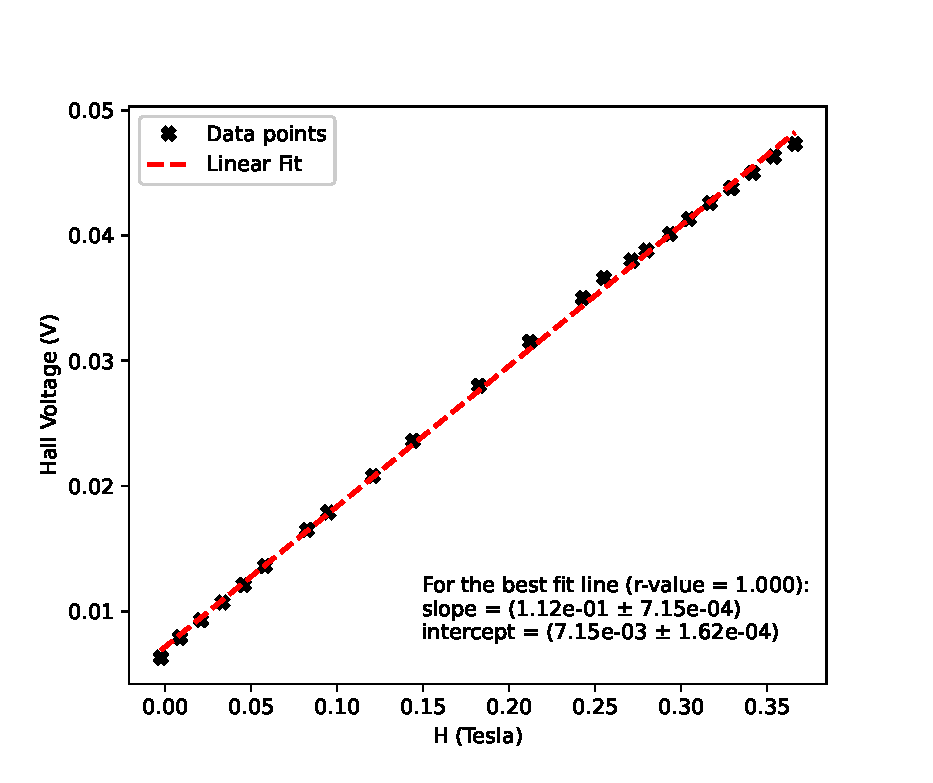
\includegraphics[width=1\columnwidth]{images/ge-p.eps}
    \caption{Hall voltage vs. Magnetic Field for Ge p-type semiconductor}
    \label{fig:geP}
\end{figure}

We can rewrite Eq. \ref{eq:1} as,

\begin{align}
    R_H = \left(\frac{V}{H}\right)\frac{t}{I}
\end{align}

where the $V/H$ is the slope of the above plot, $I$ refers to the probe current and $t$ is the thickness of the sample. Plugging in the values, the Hall coefficient comes out to be $1.300 \times 10^4$ cm$^3$/C. 

Using Eq. \ref{eq:6}, the charge carrier density comes out to be $4.81 \times 10^{14}$ cm$^{-3}$. Similarly using Eq. \ref{eq:7}, the carrier mobility $(\mu_e)$ comes out to be,
$\mu_e = R_H\sigma=R_H / 7 = 1.86 \time 10^3\text{ cm}^2/\text{Vs}$

% \begin{align*}
% \end{align*}

\subsubsection{Ge n-type}
The Hall voltage against different values of coil currents is shown in Table \ref{tab:geN}. The Hall voltage as a function of the magnetic field obtained through the calibration curve plot is shown in Fig. \ref{fig:geN}. For this setup,

\begin{itemize}
    \item Probe current = 3.88 mA
    \item Resistivity $\sigma = (7 \pm 1)\,\Omega$ cm 
    \item Sample thickness $t= 0.5$ mm\\
\end{itemize}

\noindent Note that since this is an n-type semiconductor, the majority charge carriers are electrons. Hence, the Hall voltage increases in the negative direction as opposed to the previous case. Using the same methods used for Ge p-type semiconductor, the Hall coefficient of Ge n-type comes out to be $-2.154 \times 10^4$ cm$^3$/C.

Using Eq. \ref{eq:6}, the charge carrier density comes out to be $2.90 \times 10^{14}$ cm$^{-3}$. Similarly using Eq. \ref{eq:7}, the carrier mobility $(\mu_e)$ comes out to be,
$\mu_e = R_H/7 = 3.08 \times 10^3 \text{ cm}^2/\text{Vs}$

% \begin{align*}
% \end{align*}
\begin{table}[H]
    \centering
    \begin{tabular}{|c|c|c|c|}
    \hline
    Current & Hall Voltage & Current & Hall Voltage \\ 
    (A) & (mV) & (A) & (mV) \\ \hline
    0.00 & 1.2 & 1.70 & 36.4 \\ \hline
    0.10 & 3.2 & 1.91 & 40.8 \\ \hline
    0.30 & 7.2 & 2.01 & 43.1 \\ \hline
    0.50 & 11.3 & 2.16 & 46.0 \\ \hline
    0.70 & 15.3 & 2.30 & 48.9 \\ \hline
    0.90 & 19.7 & 2.50 & 52.8 \\ \hline
    1.01 & 21.7 & 2.72 & 57.1 \\ \hline
    1.10 & 24.0 & 2.89 & 60.7 \\ \hline
    1.30 & 28.0 & 3.01 & 63.0 \\ \hline
    1.50 & 32.1 & 3.12 & 64.9 \\ \hline
    \end{tabular}
    \caption{Current supplied to the electromagnet and
    corresponding hall voltage produced for Ge n-type
    semiconductor}
    \label{tab:geN}
    \end{table}
\begin{figure}[H]
    \centering
    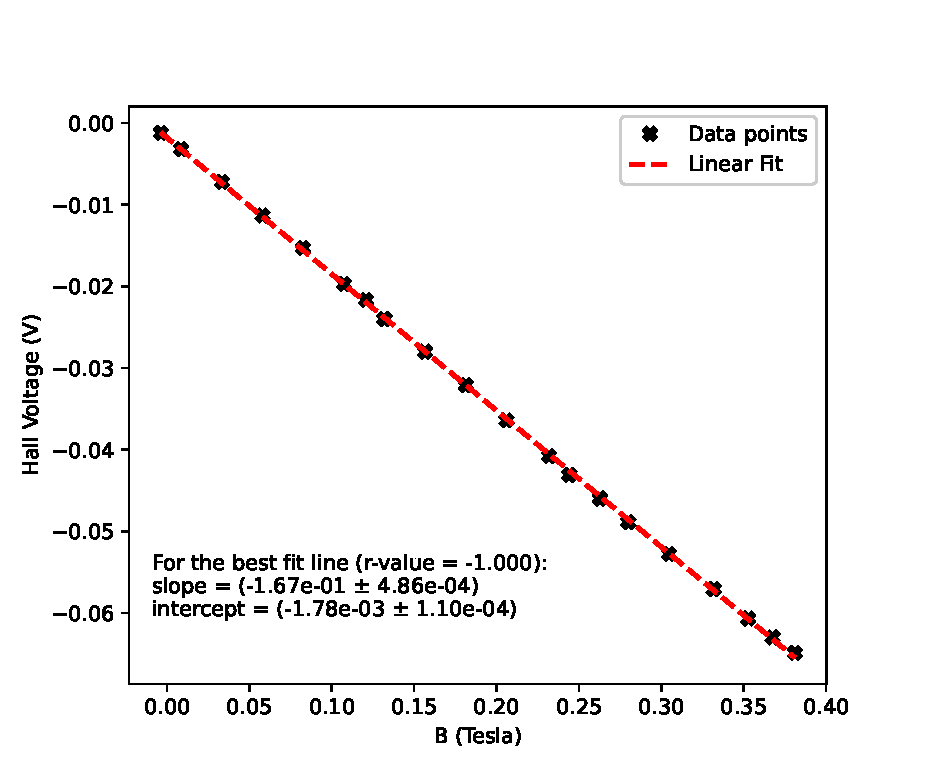
\includegraphics[width=1\columnwidth]{images/ge-n.eps}
    \caption{Hall voltage vs. Magnetic Field for Ge n-type semiconductor}
    \label{fig:geN}
\end{figure}


\subsubsection{Si n-type}
The Hall voltage against different values of coil currents is shown in Table \ref{tab:siN}. The Hall voltage as a function of the magnetic field obtained through the calibration curve plot is shown in Fig. \ref{fig:siN}. For this setup,

\begin{itemize}
    \item Probe current = 3.92 mA
    \item Resistivity $\sigma = (24 \pm 1)\,\Omega$ cm 
    \item Sample thickness $t= 0.5$ mm\\
\end{itemize}

\noindent Using the same methods used for Ge n-type semiconductor, the Hall coefficient of Ge n-type comes out to be $-1.791\times 10^3$ cm$^3$/C.

Using Eq. \ref{eq:6}, the charge carrier density comes out to be $3.49 \times 10^{14}$ cm$^{-3}$. Similarly using Eq. \ref{eq:7}, the carrier mobility $(\mu_e)$ comes out to be,
$ \mu_e = R_H / 24 = 0.75\text{ cm}^2/\text{Vs}$

% \begin{align*}
% \end{align*}
\begin{table}[H]
    \centering
    \begin{tabular}{|c|c|c|c|}
    \hline
    Current & Hall Voltage & Current & Hall Voltage \\ 
    (A) & (mV) & (A) & (mV) \\ \hline
    0 & -2.9 & 1.7 & 24.4 \\ \hline
    0.1 & -1.6 & 1.9 & 27.7 \\ \hline
    0.31 & 1 & 2.02 & 29.9 \\ \hline
    0.5 & 3.5 & 2.12 & 31.8 \\ \hline
    0.71 & 6.3 & 2.3 & 35.9 \\ \hline
    0.9 & 11.1 & 2.54 & 39.4 \\ \hline
    1 & 12.9 & 2.71 & 42.7 \\ \hline
    1.11 & 14.6 & 2.9 & 45.9 \\ \hline
    1.31 & 17.9 & 3.01 & 47.3 \\ \hline
    1.5 & 21.1 &  &  \\ \hline
    \end{tabular}
    \caption{Current supplied to the electromagnet vs. hall voltage produced for Si n-type
    semiconductor}
    \label{tab:siN}
    \end{table}

\begin{figure}[H]
    \centering
    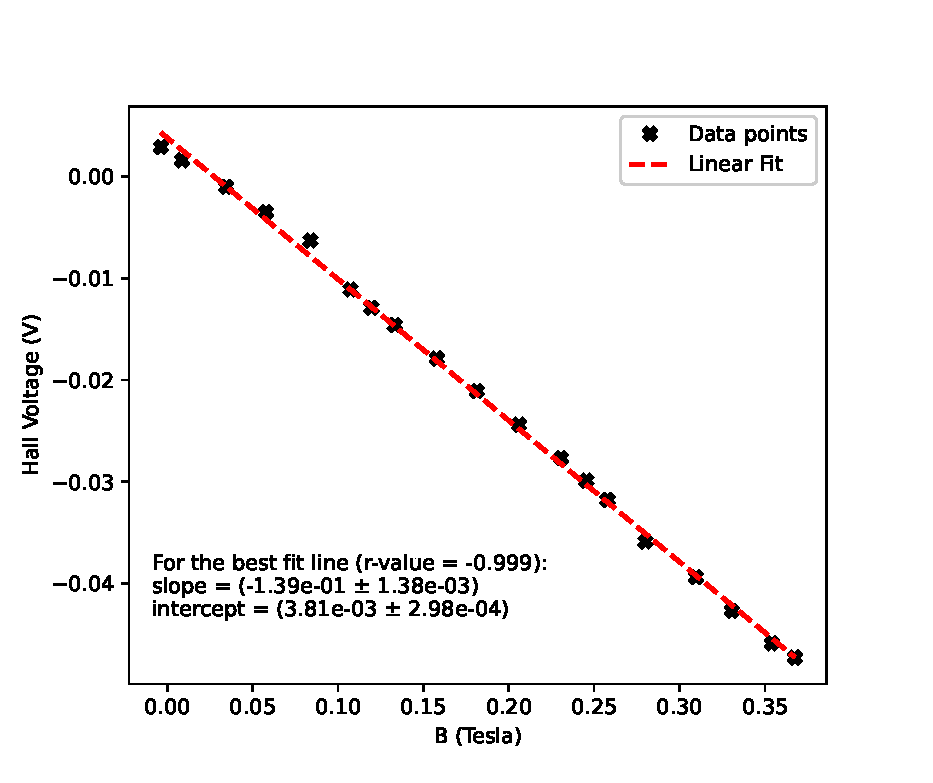
\includegraphics[width=1\columnwidth]{images/si-n.eps}
    \caption{Hall voltage vs. Magnetic Field for Si n-type semiconductor}
    \label{fig:siN}
\end{figure}

\subsection{Temperature variation of Hall Coefficient}
Using a Ge p-type semiconductor fixed with an oven, we were able to vary the temperature on the semiconductor by varying the EMF supplied to the oven. Temperature is measured with Cromel-Alumel thermocouple with its junction at a distance
of 1 mm from the crystal. After waiting for about 10 minutes after each change in thermal EMF, we measured the Hall voltage and corresponding Hall coefficient (Table \ref{tab:tem}) to obtain a relationship as shown in Fig. \ref{fig:tem}.

\begin{table*}[]
    \centering
    \begin{tabular}{|c|c|c|c|c|c|}
    \hline
    Thermal  & Temperature & Hall & Offset & Corrected Hall & Hall \\ 
    EMF (mV) & ($^\circ$C) & Voltage (mV) & Voltage (mV) & Voltage (mV) & Coefficient (cm$^3$/C) \\ \hline
    1.00 & 25.00 & 28.5 & 18.9 & 9.6 & 6.24 \\ \hline
    1.25 & 31.25 & 27.4 & 18.1 & 9.3 & 6.04 \\ \hline
    1.71 & 42.75 & 27.3 & 18.6 & 8.7 & 5.65 \\ \hline
    2.30 & 57.50 & 24.3 & 18.0 & 6.3 & 4.09 \\ \hline
    2.82 & 70.50 & 17.9 & 14.8 & 3.1 & 2.01 \\ \hline
    3.51 & 87.75 & 9.6 & 9.4 & 0.2 & 0.13 \\ \hline
    4.30 & 107.50 & 5.0 & 5.5 & -0.5 & -0.32 \\ \hline
    4.74 & 118.50 & 4.0 & 4.5 & -0.5 & -0.32 \\ \hline
    \end{tabular}
    \caption{}
    \label{tab:tem}
    \end{table*}
As we can see, the Hall coefficient is
observed to decrease with increasing temperature,
and a significant drop is seen at higher temperatures roughly after 50$^\circ$C to 70$^\circ$C. After that, it more or less stabilises.
\begin{figure}
    \centering
    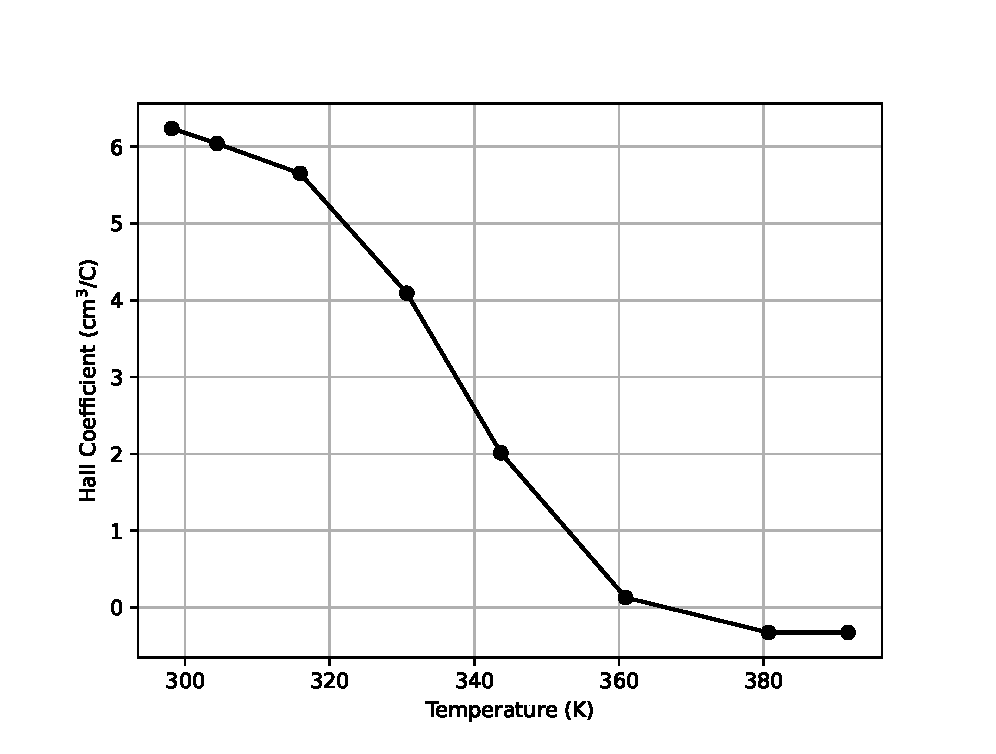
\includegraphics[width=1\columnwidth]{images/temp.eps}
    \caption{Hall voltage and coefficient measured at different temperatures for Ge p-type semiconductor}
    \label{fig:tem}
\end{figure}


This behaviour can be explained by examining the semiconductor properties at the low temperature region. Here, the conduction is primarily due to
holes (majority carriers in p-type semiconductors).
As the temperature rises, thermal energy of the particles increase,
which causes the excitation of electrons from the valence band to the conduction band. This increases the minority carrier concentration (electrons). Since Hall coefficient is inversely proportional to the difference in carrier concentrations,

\begin{align}
    R_H = \frac{1}{q(p-n)}
\end{align}

where $p$ and $n$ are the  hole and electron concentrations respectively, the overall value of $R_H$ decreases. Hence, the semiconductor transitions from an extrinsic to intrinsic conduction regime.

At even higher temperatures around 80$^\circ$C, the in
trinsic carrier concentration ($n_i$) becomes comparable to the dopant-induced carrier concentration ($p_0$). When $n_i$ dominates,
conduction is influenced by both electrons (minor-
ity carriers) and holes (majority carriers). Electrons,
having higher mobility than holes, significantly reduce the effective Hall coefficient. In the intrinsic conduction region, the equation for $R_H$ is,

\begin{align}
    R_H = \frac{1}{q(p+n)}\left(\frac{p-n}{p+n}\right)
\end{align}

As $p\approx n \approx n_i$, the value of $R_H$ sharply decreases. Moreover, after the significant drop, $R_H$ value more or less stabilises at a temperature corresponding to approximately 110$^\circ$C. This is expected as all the electrons from the valence band have been excited to the conduction band, so no further decrease of the Hall coefficient can occur.